% Innehållet i Vasungavisor 2010
%
% Kapitel "I Högan Nord"

\songchapter{Ur Törstiga Strupar}
\begin{figure}[!b]
\begin{center}
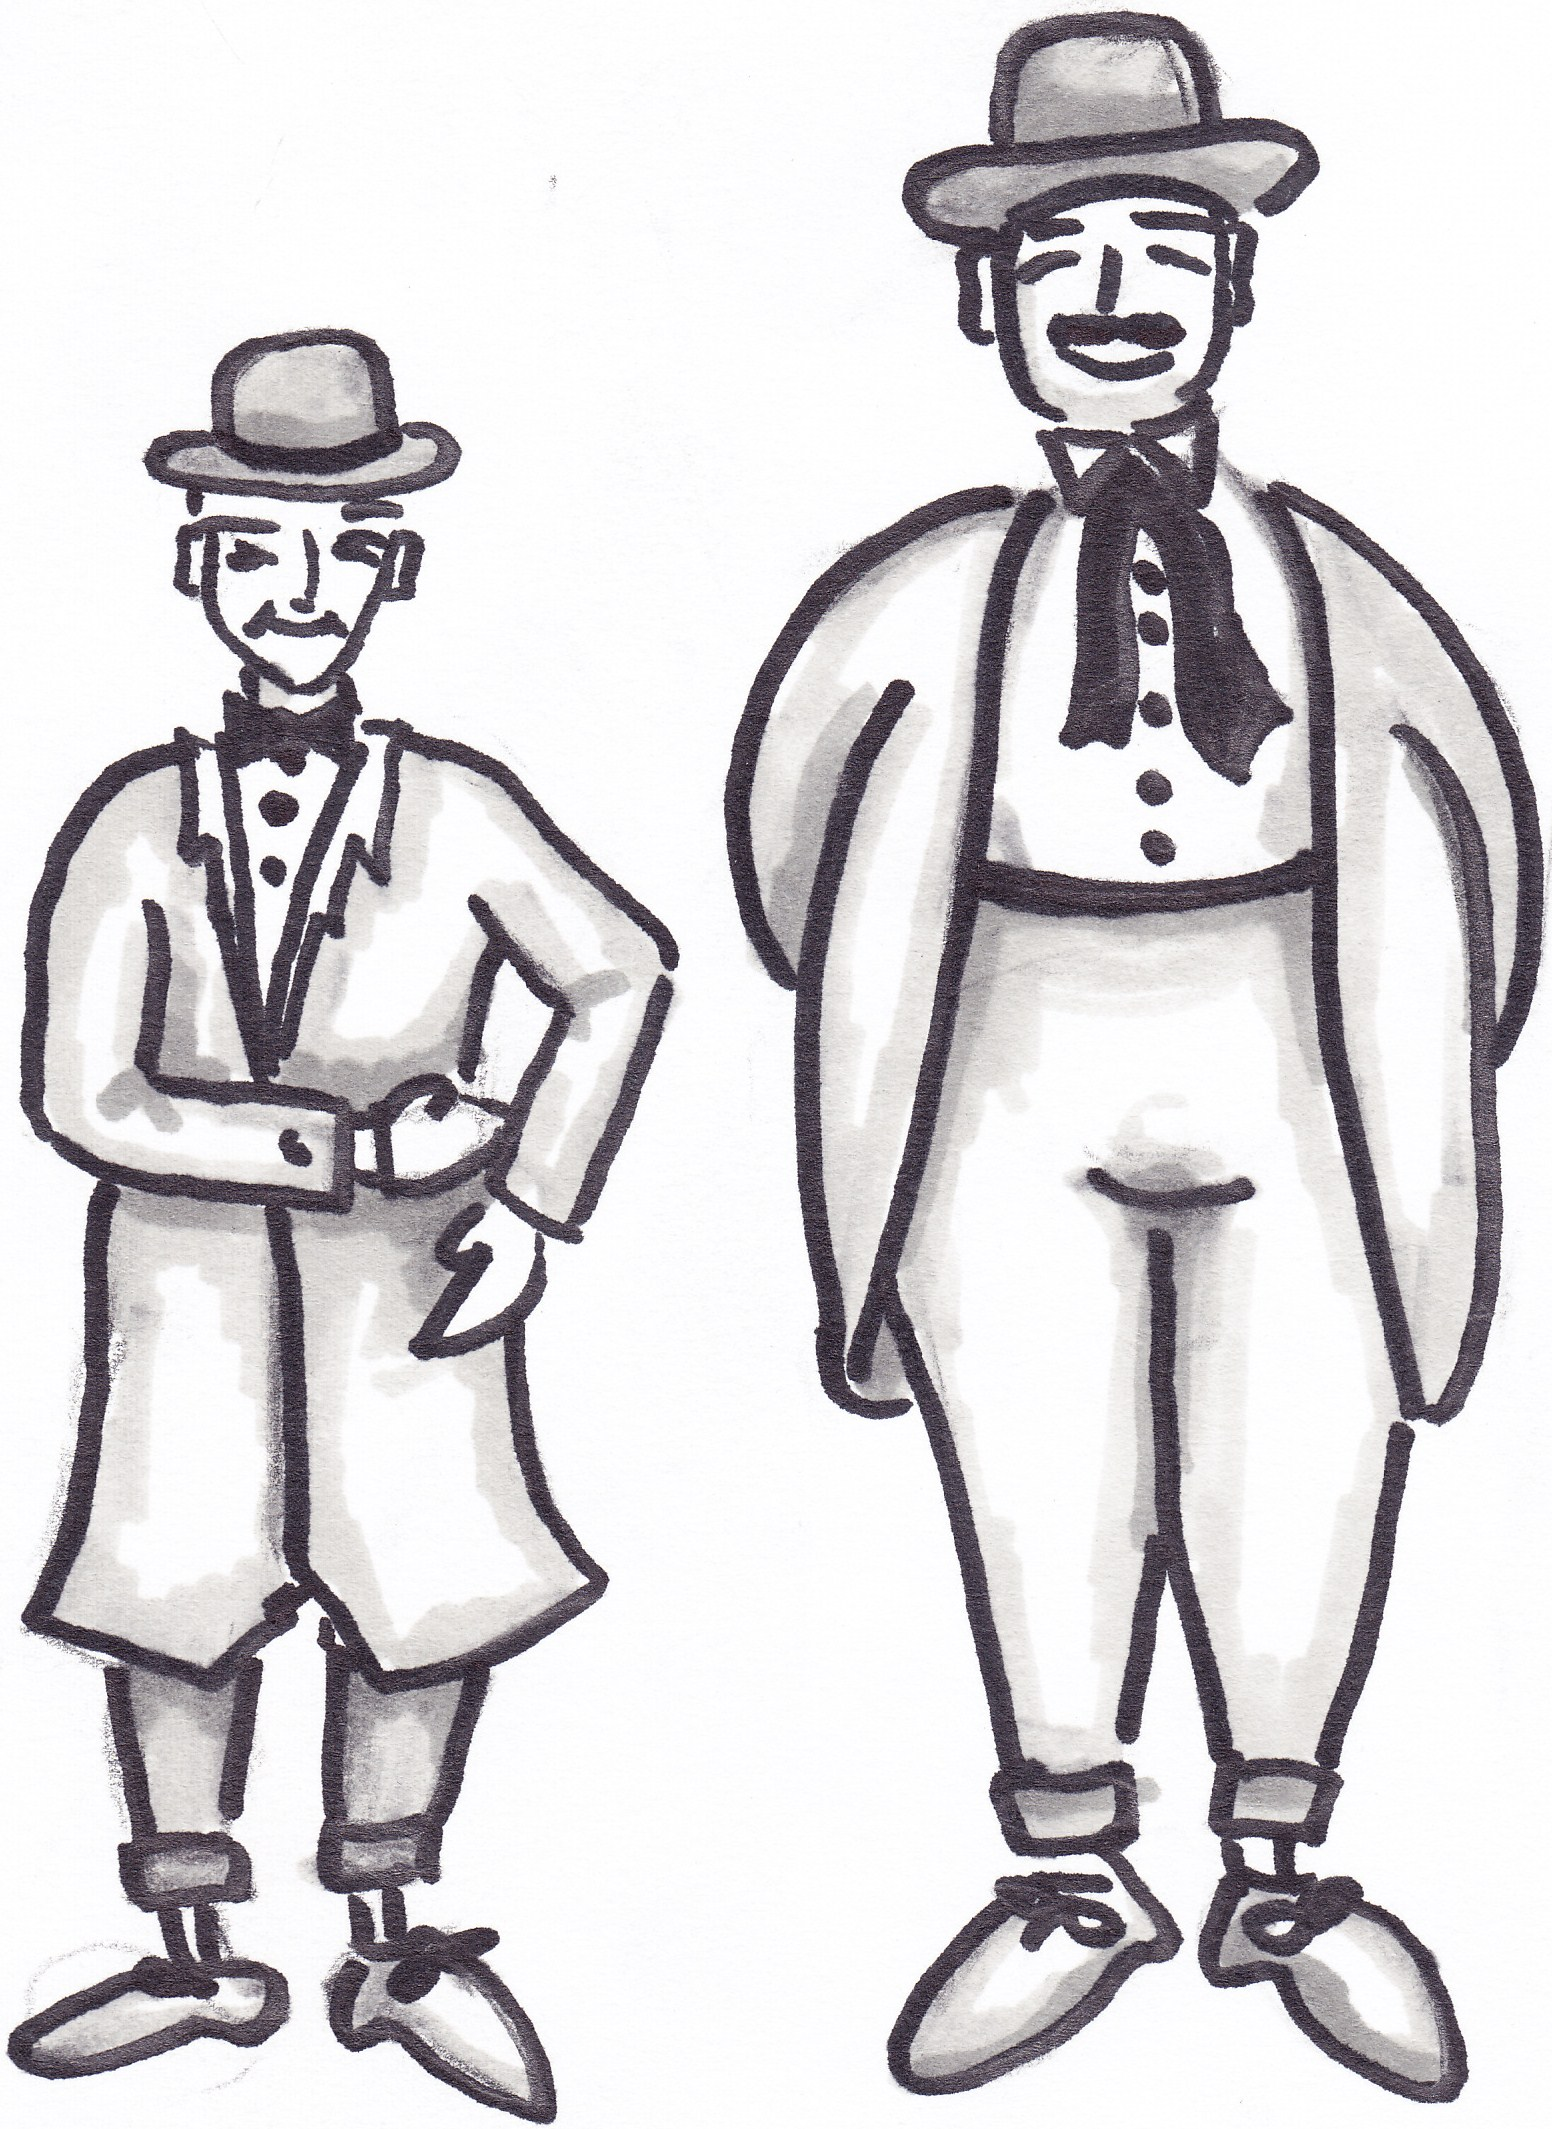
\includegraphics[width=5cm]{../bilder/helanochhalvan.jpg} 
\end{center}
\end{figure}
\clearpage
\beginsong{Helan}					
	
\beginverse*
Helan går, 
sjung hoppfaderallallallallej
helan går, 
sjung hoppfaderallallej!
Och den som inte helan tar, 
han ej heller halvan får. 
Helan går, 
sjung hoppfaderallallej!			
\endverse									
\endsong							

\beginsong{Halvan}[
		sr={Så väva vi vadmal},
		index={Så väva vi vallman}]
					
\beginverse*						
Så väva vi vallman,
så taga vi halvan.
Väva vallman och taga halvan
och låta suparna gå, gå.
\endverse		
\endsong
\beginsong{Tersen}[
		sr={},
		index={Fjärran han dröjer}]

\beginverse*						
Fjärran han dröjer ur törstiga strupar, 
redan vi tagit två modiga supar. 
Ack, lilla tersen, ack, lilla hjärtevännen, 
kommer du ej snart? Jo, jag kommer STRAX!
\endverse		
\endsong
\clearpage
\beginsong{Kvarten}[
		sr={Å jänta å ja'},
		index={Å tersen var bra}]

\beginverse*						
Å tersen var bra, å tersen var bra
och nu tar vi lilla kvarten hurra!
Å tersen var bra, å tersen var bra
och nu tar vi lilla kvarten.
När man den lilla tersen har fått,
smakar den lilla kvarten så gott,
och den smaken har vi aldrig försmått.
Hipp, hipp hurra för Småttin!
\endverse		
\endsong
\beginsong{Kvinten}					
	
\beginverse*
GE MIG TEXT!!!
\endverse									
\endsong							

\clearpage
\beginsong{Halvankaren}[ 		
	index={Och än går det vågor}]		
	
\beginverse*						
Och än går det vågor i halvankaren,
i halvankaren, i halvankaren.
Och än går det vågor i halvankaren,
i halvankaren går det vågor än.
Och så rullar vi på kuttingen igen min vän.
Det går vågor än uti halvankaren.
Och så rullar vi på kuttingen igen min vän.
Det går vågor än i den.
\endverse										
\endsong		

\beginsong{Den sällskapssjuka halvan}[ 		
	by={Stig Olin},					
	sr={Jag tror på sommaren},					
	index={När fiskargubben satt}]	
	
\beginverse*						
När fiskargubben satt på krog,
med vännerna och helan tog.
Då sa' dom: ``Ta me' samma en,
med tanke på ditt andra ben.''
Och gubben tog då halvan sin
men sade se'n med häpen min:
``Den jäkeln var en listig en,
för tänk – den gick i samma ben!''
\endverse										
\endsong		

\clearpage
\beginsong{Det satt en mås}[				
    sr={När månen vandrar},					
	index={Skärgårdsidyll},
	index={Måsen}]		
	
\beginverse*						
Det satt en mås på en klyvarbom 
och tom i krävan var kräket. 
Och tungan lådde vid skepparns gom 
där han satt uti bleket. 
Jag vill ha sill! 
hördes måseropet 
och skepparn svarte: jag vill ha O.P. 
om blott jag får, om blott jag får.
\endverse						


\beginverse				
Nu lyfter måsen från klyvarbom 
och vinden spelar i tågen. 
O.P.'n svalkat har skepparns gom, 
jag önskar blott att jag såg'en. 
Så nöjd och lycklig den arme saten, 
han sätter storsegel den krabaten, 
till sjöss han far och halvan tar!

\endverse				
\endsong		

\begin{figure}[!b]
\begin{center}
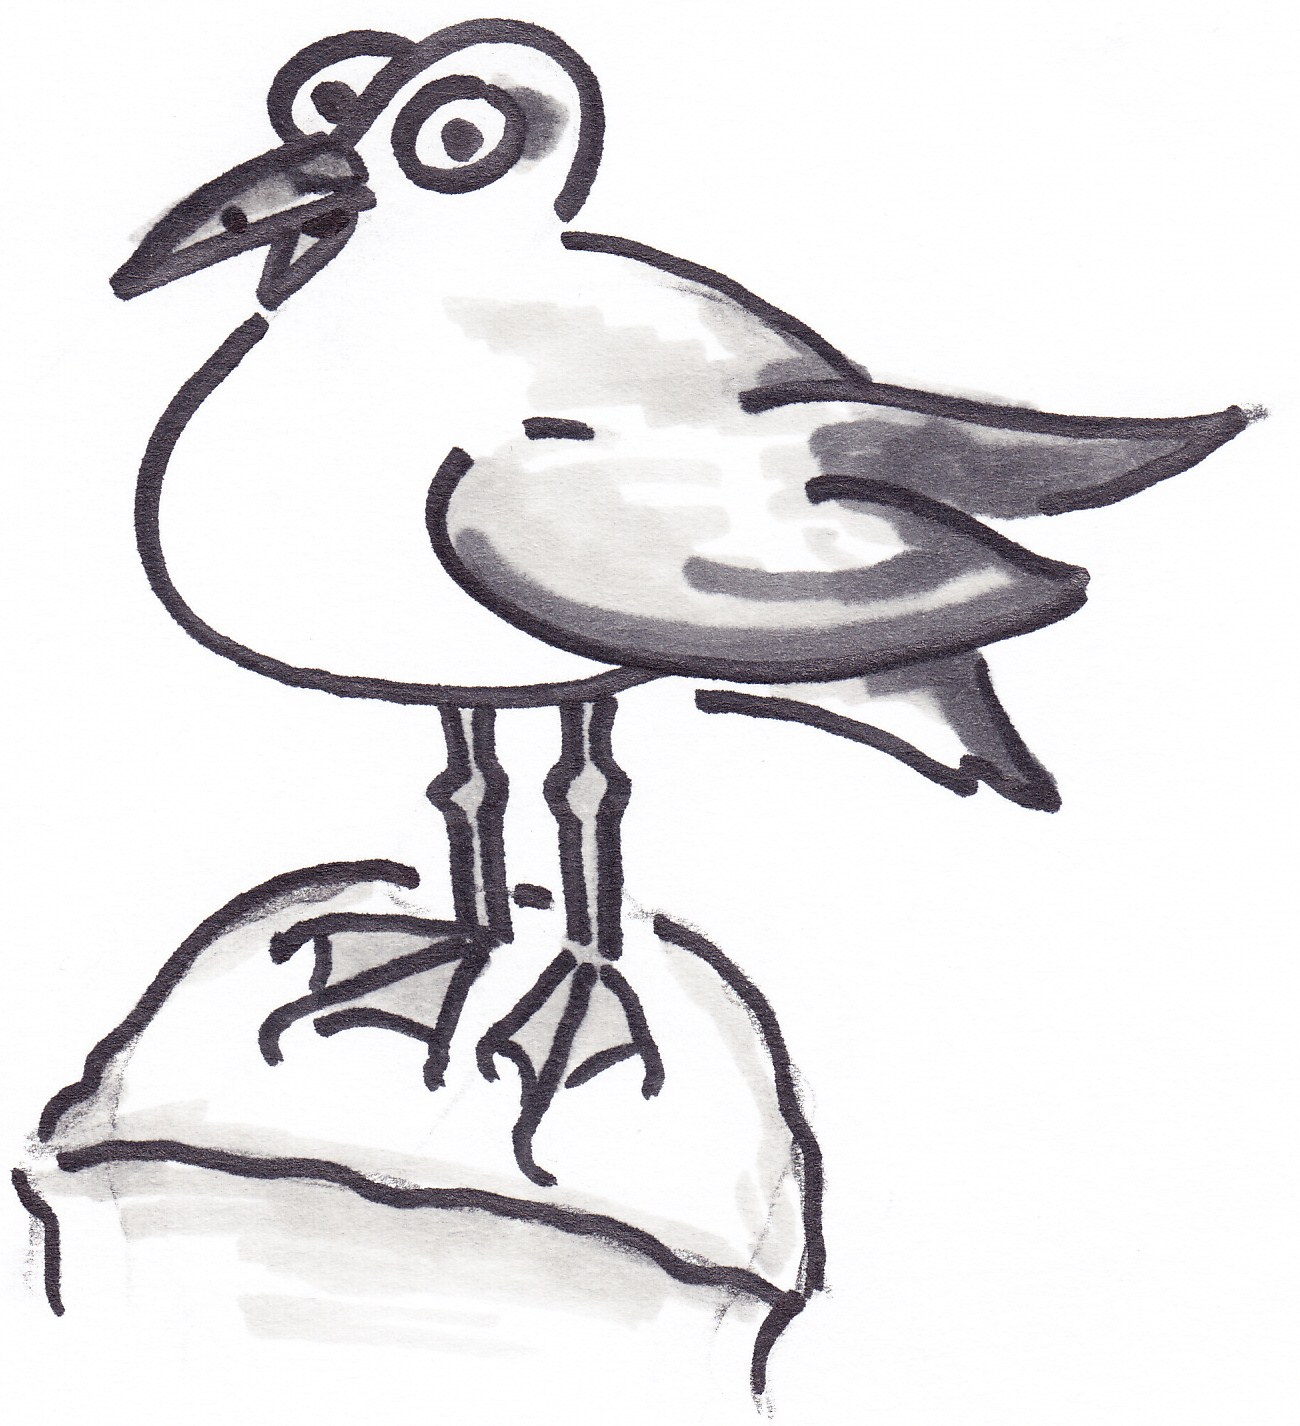
\includegraphics[width=25mm]{../bilder/mas.jpg} 
\end{center}
\end{figure}
\clearpage
\beginsong{Gå på fest}[ 							
	sr={Du ska få min gamla cykel},					
	index={När som livet kännes},
	index={Är du vissen}]		
	
\beginverse*						
När som livet kännes mörkt och grått och trist,
GÅ PÅ FEST
När humöret allt emedan du mist,
GÅ PÅ FEST
När du tror att allting grånar, 
ska du se att himlen blånar, 
sommarens blommor dig förvånar, 
GÅ PÅ FEST!
\endverse						

\beginverse				
Är du vissen, klen och trött och matt och svag, 
GÅ PÅ FEST
Skulle hjärtat bara slå vartannat slag, 
GÅ PÅ FEST
Strunt i doktorn och recepter, 
medicin och farmacepter, 
sluta upp och känna efter, 
GÅ PÅ FEST!
\endverse				
\endsong		

\clearpage
\beginsong{Härjarvisan}[ 	
    by={Hasse Alfredsson},						
	sr={Gärdebylåten},					
	index={Nu ska vi ut och härja}]		

\beginverse*
Liksom våra fäder vikingarna i Norden,
drar vi landet runt och super oss under borden.
Brännvinet har blitt ett elexir 
för kropp såväl som själ.
Känner du dig liten och ynklig på jorden,
växer du med supen och blir stor uti orden.
Slår dig för ditt håriga bröst,
och blir en man från hår till häl.
\endverse

\beginchorus				
Ja, nu skall vi ut och härja,
supa och slåss och svärja,
bränna röda stugor, slå små barn
 och säga fula ord!
Med blod skall vi stäppen färga.
Nu äntligen lär jag
kunna dra nån riktig nytta av min Hermodskurs i mord! 
\endchorus	

\beginverse					
Hurra, nu skall man äntligen få röra på benen,
hela stammen jublar och det spritter i grenen.
Tänk att än en gång få spränga fram
 på Brunte i galopp!
Din doft, o kära Brunte är trots brist i hygienen,
för en vild mongol minst lika ljuv som syrenen.
Tänk att på din rygg få rida runt
 i stan och spela topp. 
\endverse						

\beginchorus				
Ja, nu skall vi ut och härja ...
\endchorus	

\beginverse
Ja, mordbänder är klämmiga, ta fram fotogenen!
Och eftersläckningen tillhör just de fenomenen
inom brandmansyrket, som jag tycker det är nån nytta med.
Jag målar för mitt inre upp den härliga scenen: 
blodrött mitt i brandgult. Ej ens prins Eugen en
lika mustig vy kan måla, ens om han målade med sked. 
\endverse	

\beginchorus	
Ja, nu skall vi ut och härja ... 
\endchorus	
\endsong		

\beginsong{Fordom odlade man}[ 		
	sr={Vintern rasat}]		
	
\beginverse*						
Fordom odlade man vindruvsranka,
av vars frukt man gjorde ädelt vin.
Nu man pressar saften ur en planka,
doftande som äkta terpentin.
Höj din bägare, o broder, syster.
Låt den finska skogen rinna kall
nedför strupen och om du är dyster,
låt oss supa upp en liten tall
Låt oss supa upp en liten tall
Låt oss supa upp en liten tallSKOG!
\endverse										
\endsong		

\clearpage
\beginsong{Heppeneppetepp}[ 						
	index={Till Stockholm for}]		
	
\beginverse*						
Till Stockholm for Heppeneppetepp, 
till Stockholm for jag.
Till Stockholm for Heppeneppetepp,
till Stockholm for jag.
\endverse	
\beginchorus
:,: Till Stockholm for Amalia
som bad oss supa bra, 
och till Stockholm for alla raska gossar
som i laget där var. :,:
\endchorus		

\beginverse				
Och supen tog Heppeneppetepp
och supen tog jag.
Och supen tog Heppeneppetepp
och supen tog jag.
\endverse	
\beginchorus
:,: Och supen tog Amalia... :,:
\endchorus	

\beginverse
I finkan kom Heppeneppetepp
i finkan kom jag. 
I finkan kom Heppeneppetepp
i finkan kom jag.
\endverse	
\beginchorus
:,: I finkan kom Amalia... :,:
\endchorus

\beginverse
Men frikänd blev Heppeneppetepp
och frikänd blev jag. 
Men frikänd blev Heppeneppetepp
och frikänd blev jag. 
\endverse	
\beginchorus
:,: Och frikänd blev Amalia... :,:
\endchorus	
\endsong		

\clearpage


\beginsong{Hur länge skall på bordet}[
	index={Det ärvda vikingsinne}]		
	
\beginverse*						
Hur länge skall på bordet
den lilla halvan stå?
Skall snart ej höras orden:
Låt halvan gå, låt gå!
Det ärvda vikingasinne till supen trår igen 
Och helans trogna minne i halvan går igen. 
\endverse									
\vspace{5mm}
\endsong		

\beginsong{Det perfekta glaset}[
	by={Nicklas Forss},
	sr={Sommardag i Kangasala},
	index={Jag lyfte den lilla supen}]
	
\beginverse*						
Jag lyfte den lilla supen
och hällde den i min hals.
Det kittla så härligt i strupen,
men kvar fanns sen inget alls.
Jag titta på glaset och drömde
att det hade sådan funktion:
:,: hur mycket man än ur det tömde,
där alltid fanns kvar en portion. :,:
\endverse						
\endsong		

\clearpage
\beginsong{Kassen full}[				
	sr={Vinden drar}]		
	
\beginverse*						
Kassen full
förbi vår tull
hämtar jag hem med mig.
Jag hämtar brännvin, genever och gin
och allt så dricker jag själv. 
\endverse		
		
\vspace{5mm}
\endsong		

\beginsong{Infinitesimaldifferensen}[ 							
	sr={Hipp-hurra för Bamsefar},					
	index={Enligt Darwins teori}]		
	
\beginverse*						
Enligt Darwins teori
dag för dag utvecklas vi.
Men varför har vi högre rang
än Zoos orangutang?
\endverse						

\beginchorus
Jo, djuret vid sitt vattenhål
ser till vätskebalansen
och endast primitiva vrål
kan höras från seansen.
Men människan, ett högre djur,
tar glaset med förtjusning.
Hon sjunger uti moll och dur,
och dricker för berusning.
\endchorus

\beginverse				
Tänk på enda skillnaden,
så du respekterar den!
Tag dig därför ingen tår
om du ej kan ``Helan går''!
\endverse				
\endsong		

\clearpage
% Exempel på färdig-formaterad sång till VN:s
% sångbok 2010.

% Denna fil kan användas som sådan, bara verserna,
% namnen och annan rådata behöver bytas ur fälten.
% Tecknet "%" markerar en kommentar som helt och 
% hållet ignoreras av programmet som läser filen.

% Spara den färdiga filen som 
% 'SangnamnUtanMellanslagEllerSkander.tex'
% t.ex. blir "Vid En Källa" till 
% 'VidEnKalla.tex'
% Varje sång blir en egen fil.

\beginsong{Jag har aldrig vart på snusen}[ 	% Börja sången här
	by={},	% Författare
	sr={O hur saligt att få vandra}]		% Alternativa
			% sångnamn
	
\beginverse*		% Börja vers
Jag har aldrig vatt på snusen,
aldrig rökat en cigarr - halleluja!
Mina dygder äro tusen,
inga syndiga laster jag har.
\endverse
\beginverse*
Jag har aldrig sett nå't naket,
inte ens ett litet nyfött barn.
Mina blickar går mot taket,
därmed undgår jag frestarens garn.
\endverse			% Sluta vers

\beginchorus
Halleluja, halleluja, 
halleluja, halleluja
halleluja, halleluja,
Hallelujaaa-aaa-a!
\endchorus

\beginverse*		% Börja vers
Bachus spelar på gitarren,
Satan spelar på sitt handklaver.
Alla djävlar dansar tango,
säg vad kan man väl önska sig mer?
\endverse
\beginverse*
Jo, att alla bäckar vore brännvin,
stadsparksdammen full av bayerskt öl,
konjak i varenda rännsten
och punsch i varendaste pöl.
\endverse			% Sluta vers

\beginchorus
Halleluja, halleluja...
\endchorus
\endsong			% Sluta sång

\clearpage
\beginsong{Kosmonauten}[ 						
	sr={Sovjetunionens nationalsång},					
	index={Mitt namn är Nikolajev},
	index={Jag längtar hem}]		
	
\beginverse*						
Mitt namn är Nikolajev, 
kosmonaut ifrån Sovjet. 
Jag flyger runt jorden i min rymdraket. 
Och jag ska vara oppe i åttifyra varv, 
för det har Krusse sagt,
men det tycker jag är larv. 
\endverse						

\beginchorus				
Jag längtar hem, hem till min planet,
bom- bom,
till fru och barn, där hemma i Sovjet,
bom- bom.
Men mest av allt längtar jag till ett rum, 
med ett hjärta på dörrn,
bom- bom.
Ja, jag längtar hem till min planet, 
till fru och barn, därhemma i Sovjet. 
\endchorus	

\beginverse
Min kapsel innehåller många instrument,
ja, mycket av sådant som ännu ej är känt. 
Men lika förbannat, vad ni än nu tror, 
jag glömde gå på muggen innan jag for.
\endverse	

\beginchorus
Jag längtar hem...
\endchorus		
\endsong		

\begin{figure}[!t]
\begin{center}
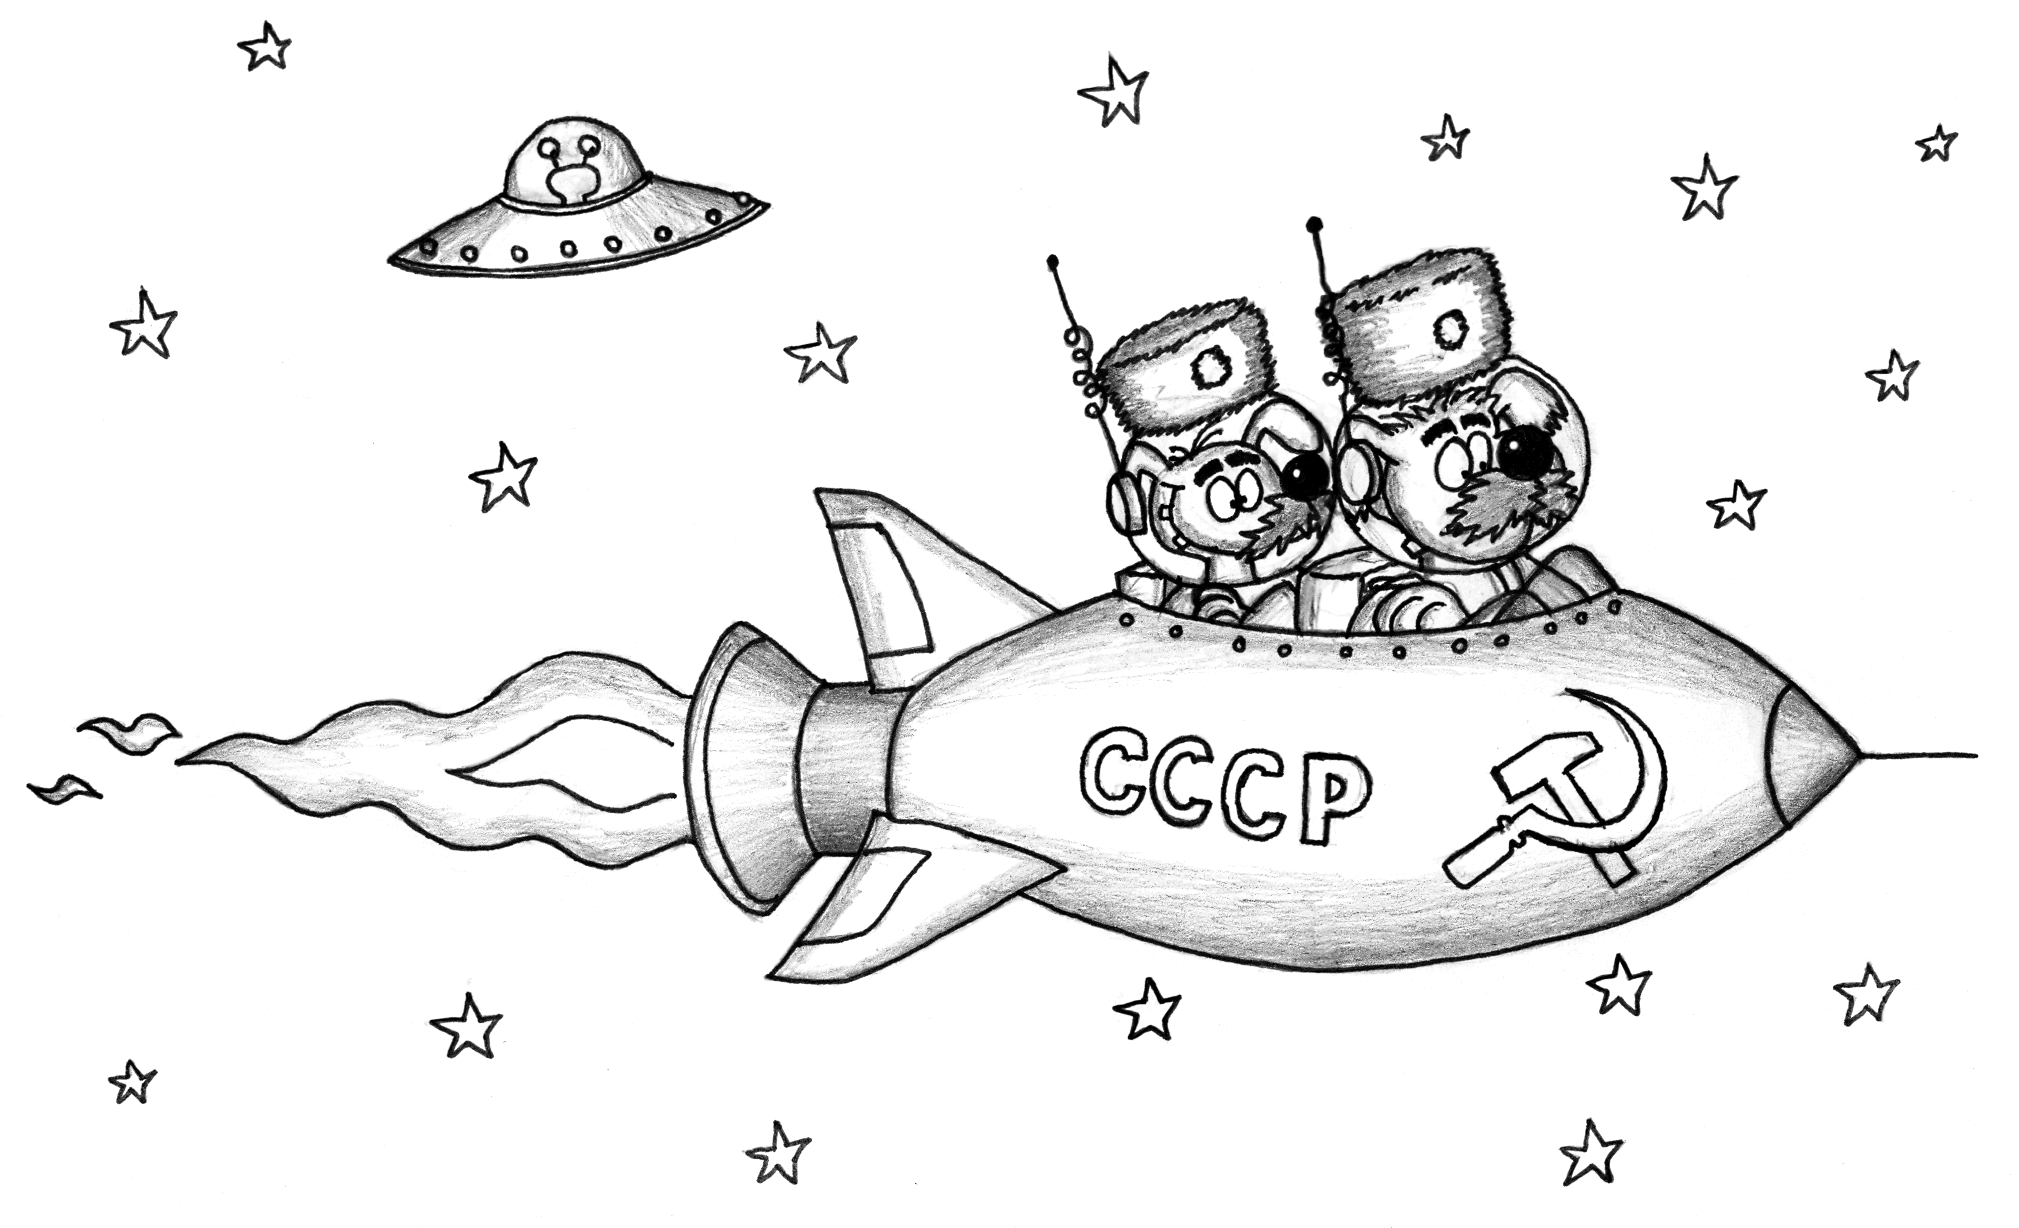
\includegraphics[width=6cm]{../bilder/kosmonauten.png} 
\end{center}
\end{figure}
\vspace{25mm}
\beginsong{Mitt lilla lån}[ 						
	sr={Hej tomtegubbar}]	
	
\beginverse*						
:,: Mitt lilla lån det räcker inte, det går till öl och till brännvin! :,:
Till öl och brännvin går det åt, 
och så till flickor emellanåt.
Mitt lilla lån det räcker inte, 
det går till öl och till brännvin
\endverse				
\endsong		

\clearpage
\beginsong{Livet är härligt}[ 							
	sr={Pråmdragarna på Volga},
	index={Ta dig en vodka}]		
	
\beginverse*						
Livet är härligt,
tavaritj, vårt liv är härligt!
Vi alla våra små bekymmer glömmer, 
när vi har fått en tår på tand; en skål!,
\endverse						

\beginverse				
Ta dig en vodka, 
tavaritj, en liten vodka! 
Glasen i botten vi tillsammans tömmer,
det kommer mera efter hand; en skål!
\endverse				
\endsong		

\begin{figure}[!b]
\begin{center}
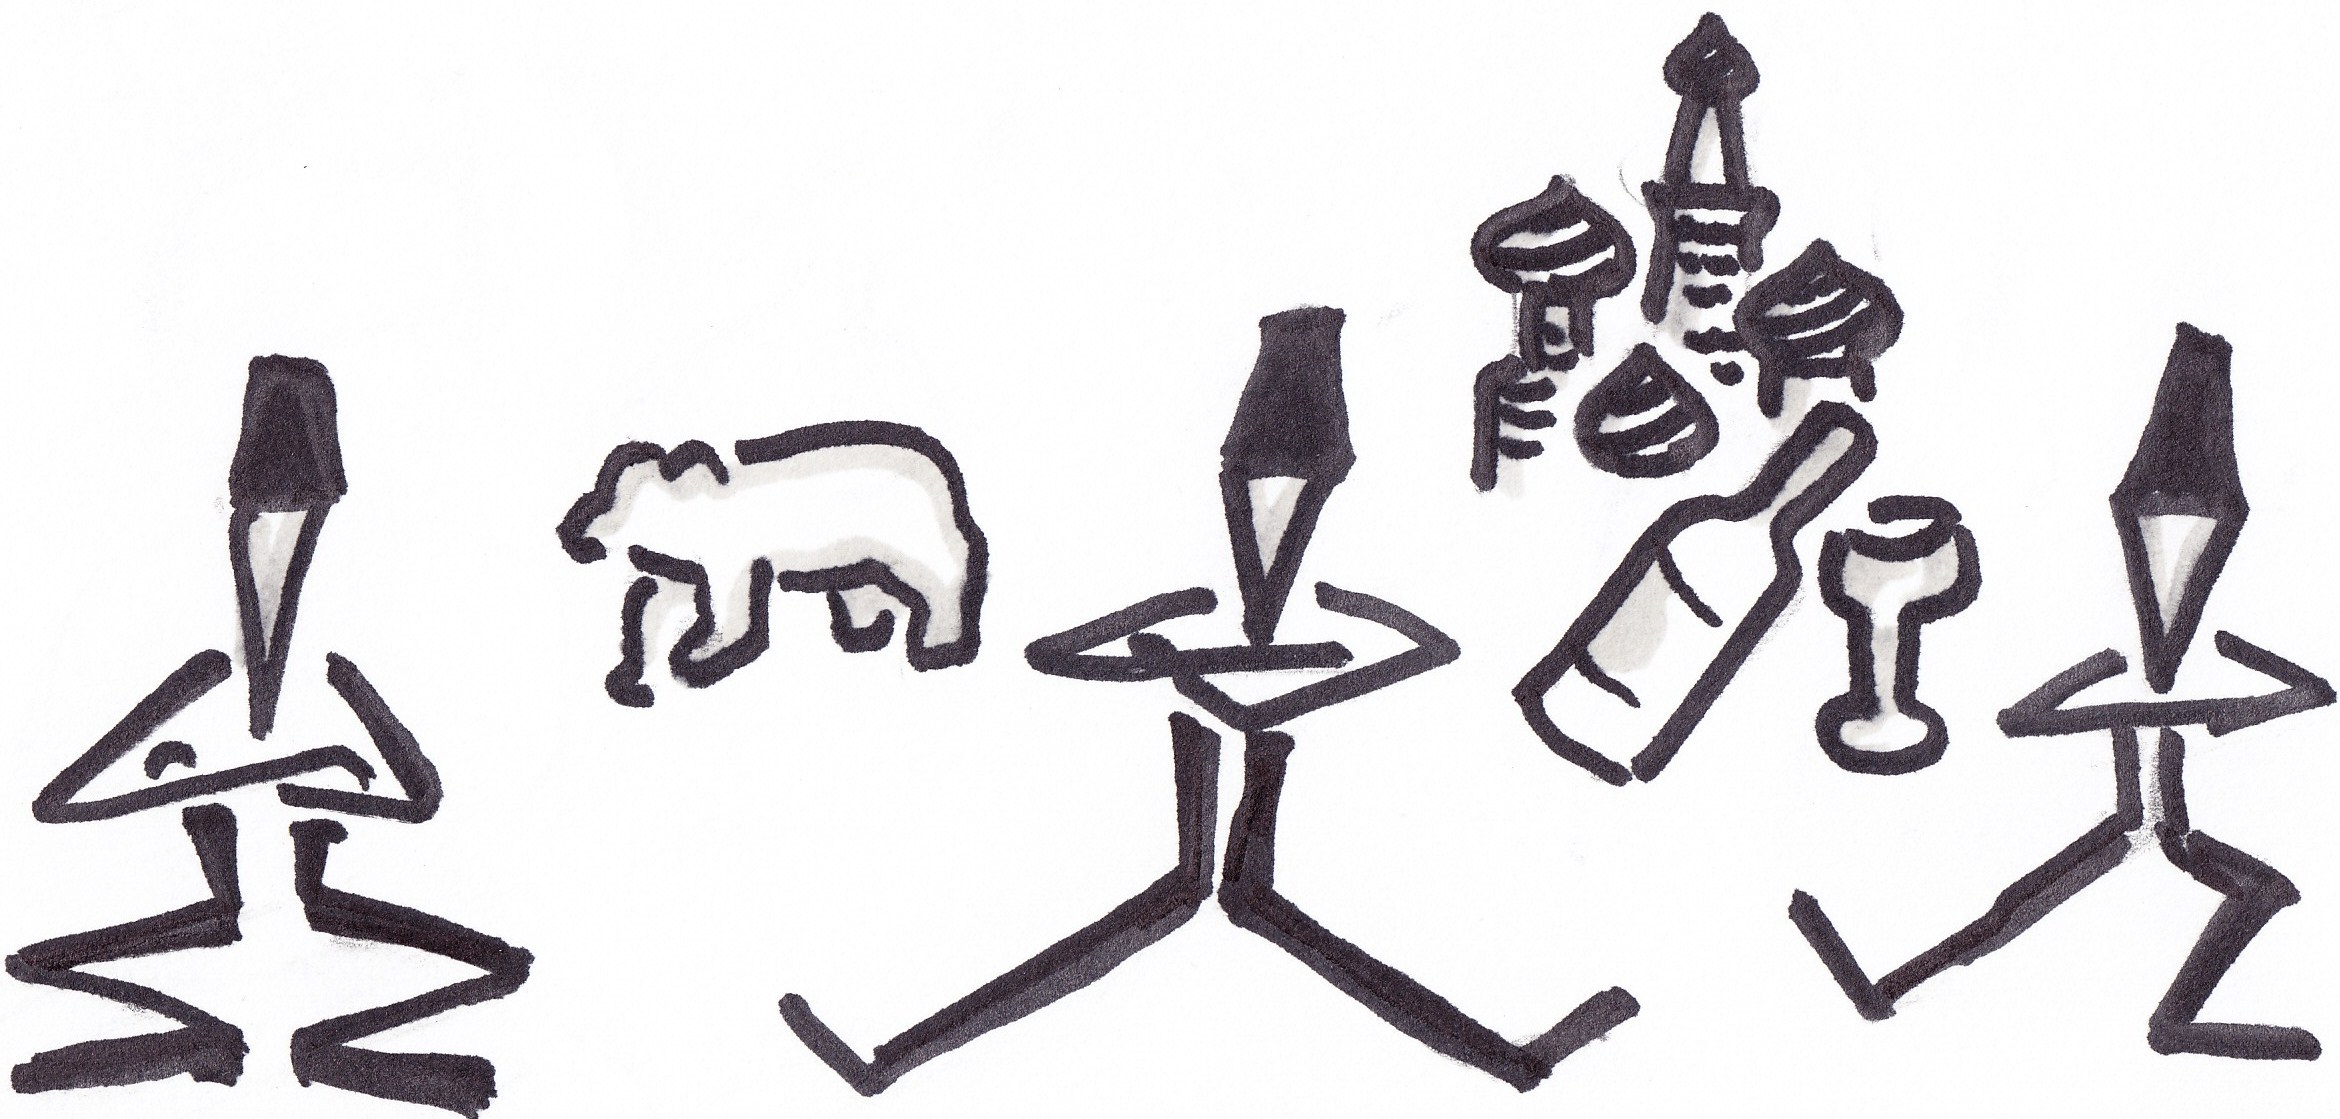
\includegraphics[width=6cm]{../bilder/livet_ar_harligt.jpg} 
\end{center}
\end{figure}
\clearpage
\beginsong{Mera brännvin}[ 						
	sr={Internationalen},					
	index={Internationalen}]		
	
\beginverse*						
Mera brännvin i glasen,
mera glas på vårt bord,
mera bord på kalasen,
mer kalas på vår jord.
\endverse						

\beginverse				
Mera jordar kring månen,
mera måne i mars,
mera marscher till Skåne,
mera Skåne - bevars!
\endverse			

\vspace{1cm}	
\endsong		

\beginsong{Om cykling}[ 		
	by={Povel Ramel},					
	sr={Så väva vi vallman},					
	index={Man cyklar för litet}]		
	
\beginverse*						
Man cyklar för litet, 
man röker för mycket.
Och man är fasen så liberal 
när det gäller maten och spriten. 
Man borde slutat för länge sedan
men denna sup är så liten. 
Vad tjänar att hyckla? 
Tids nog får man cykla! 
\endverse										
\endsong		

\clearpage
\beginsong{Minnet}[ 		
	by={T. Perret},					
	sr={Memories}]		
	
\beginverse*						
Minne! 
Jag har tappat mitt minne! 
Är jag svensk eller finne? 
Kommer inte ihåg.
Inne!
Är jag ut eller inne? 
Jag har luckor i minne, 
sån' där små alkohål. 
Men besinn' er, 
man tätar med det brännvin man får, 
när som minnet och helan går. 
\endverse						

\beginverse				
Minne!
Muisti hävis mut minne,
kunhan selvittäisimme
mitä sattunut on.
Minne!
Lähtisin vaikka minne,
juhlista selvisimme,
muistikatkoja on.
Mutta tiedän,
minä keinon mikä
auttapi tuo.
Ota ryyppy,
ja muistis juo.
\endverse				
\endsong		

\clearpage
\beginsong{Presidentvisan}[ 							
	sr={Och jungfrun hon går i ringen},					
	index={Och Mauno han satt på Gullranda}]		
	
\beginverse*						
Och Mauno han satt på Gullranda,
hojta på frun.
Men frun satt i andra ändan
ut i sitt paulun.
Det eka' i valven som vette mot norr,
när Mauno gick till skåpet
för att ta sig en knorr.
\endverse						

\beginverse				
``Kom hit, ska vi ta en tuting,
fru Tellervo!''
Men Tellervo skrek tillbaka:
``Nej, Mauno, nå, nå!''
Men avståndet gör att man kan vara viss,
att Mauno han svälja och säga:``KIPPIS!''
\endverse				
\endsong		

\begin{figure}[!b]
\begin{center}
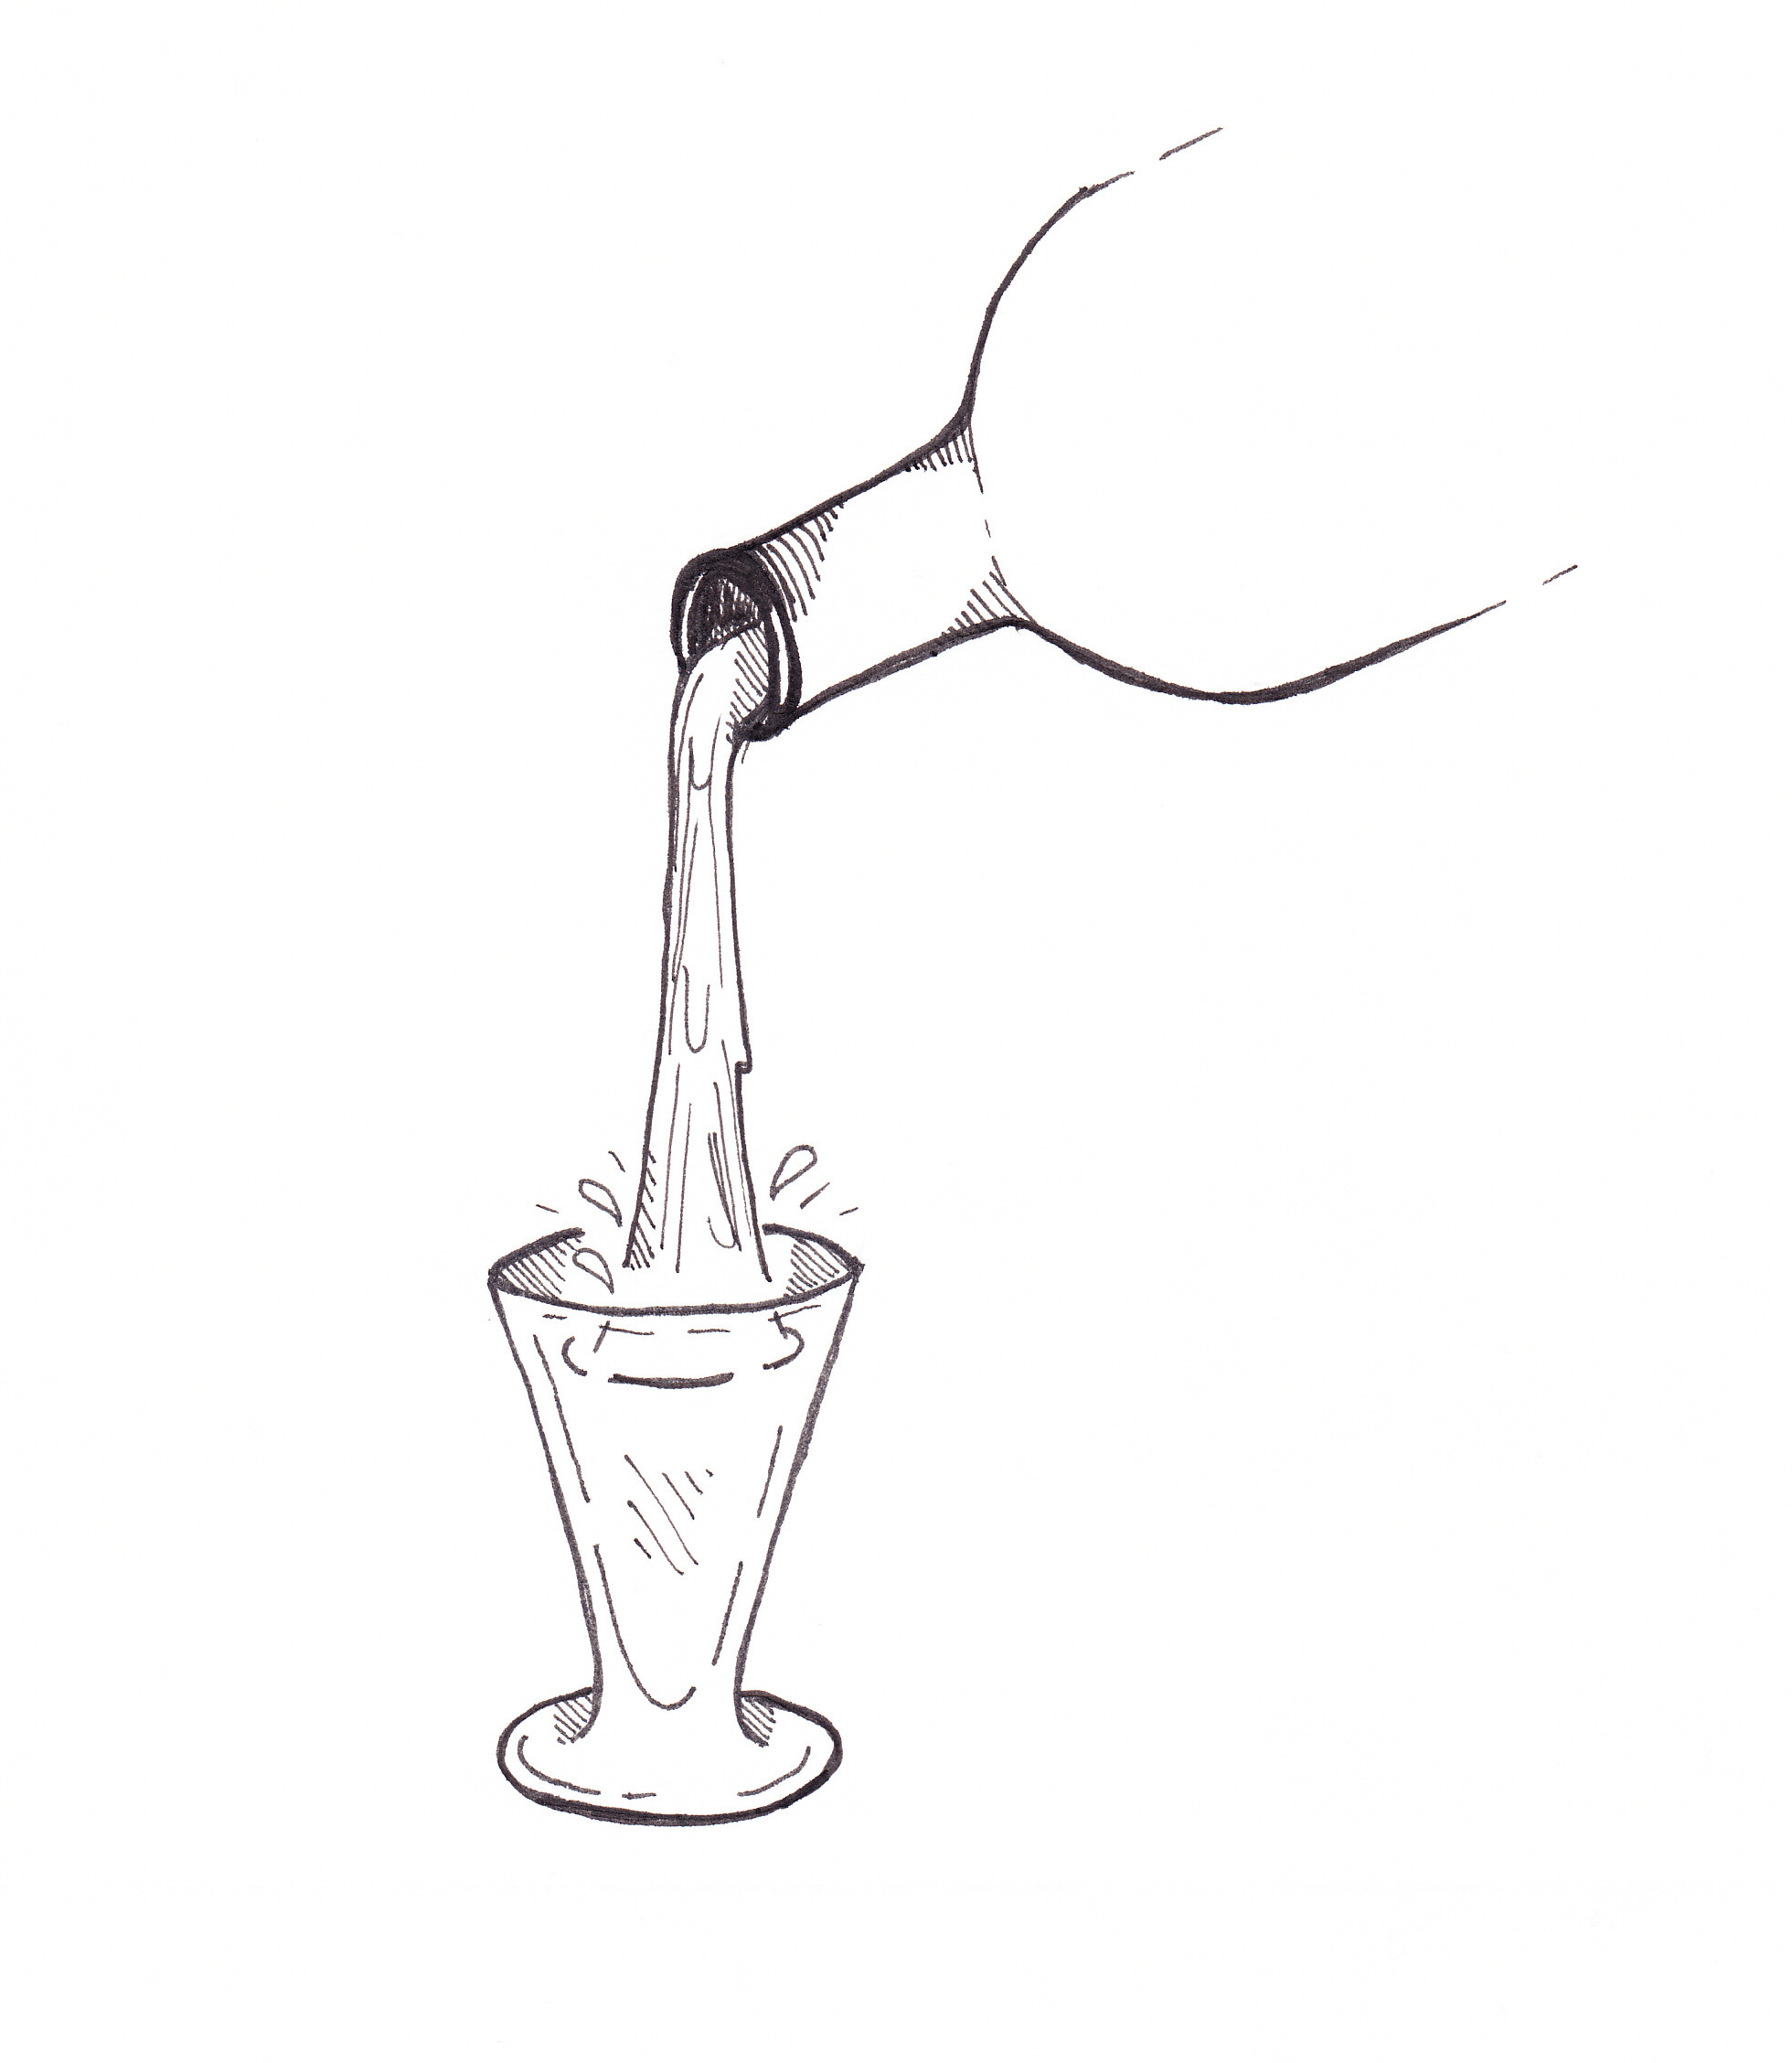
\includegraphics[width=30mm]{../bilder/hallandeflaska.jpg} 
\end{center}
\end{figure}
\clearpage
\beginsong{Rattataa}[
	index={Att dricka brännvin}]		
	
\beginverse*						
Att dricka brännvin är en sed
som ingen har oss lärt.
Från början vi ej kunde 
men det var blott temporärt.
Vi lärde oss så småningom
det var nog värt besvärt.
Tittilurenbom, tutidalenpang,
det var nog värt besvärt.
\endverse						

\beginchorus				
:,: Rattataa, så tar vi oss en tuting,
rattataa, med mycket brännvin i.
Rattataa, rattataa
dricka brännvin gillar ja'
för jag blir så full och gla’. :,:
\endchorus				
\endsong		

\clearpage
\beginsong{Ren helan slunkit ner}[
	index={Så drickom, drickom}]		
	
\beginverse*						
Ren helan slunkit ner 
och halvan tagen är, 
men magen vill ha mer, 
men magen vill ha mer, 
ej släckt är dess begär. 
Till tersen nu den trår, 
till tersen nu den trår. 
Så drickom, drickom, skål gutår.
\endverse										
\endsong		

\clearpage
\beginsong{Brännvin, vatten}[ 	
	by={Atte och Jocke Boström},					
	index={Viinaa, vettä}]		
	
\beginverse*						
Brännvin, vatten,
 smakar skit som katten. 
Brännvin, helt rått,
 :,: smakar jävligt gott! :,:
\endverse
						
\beginverse				
Viinaa, vettä 
- mitä perkelettä? 
Viinaa raakaa 
:,: napaan kaatakaa! :,:
\endverse			

\vspace{1cm}	
\endsong		

\begin{figure}[!b]
\begin{center}
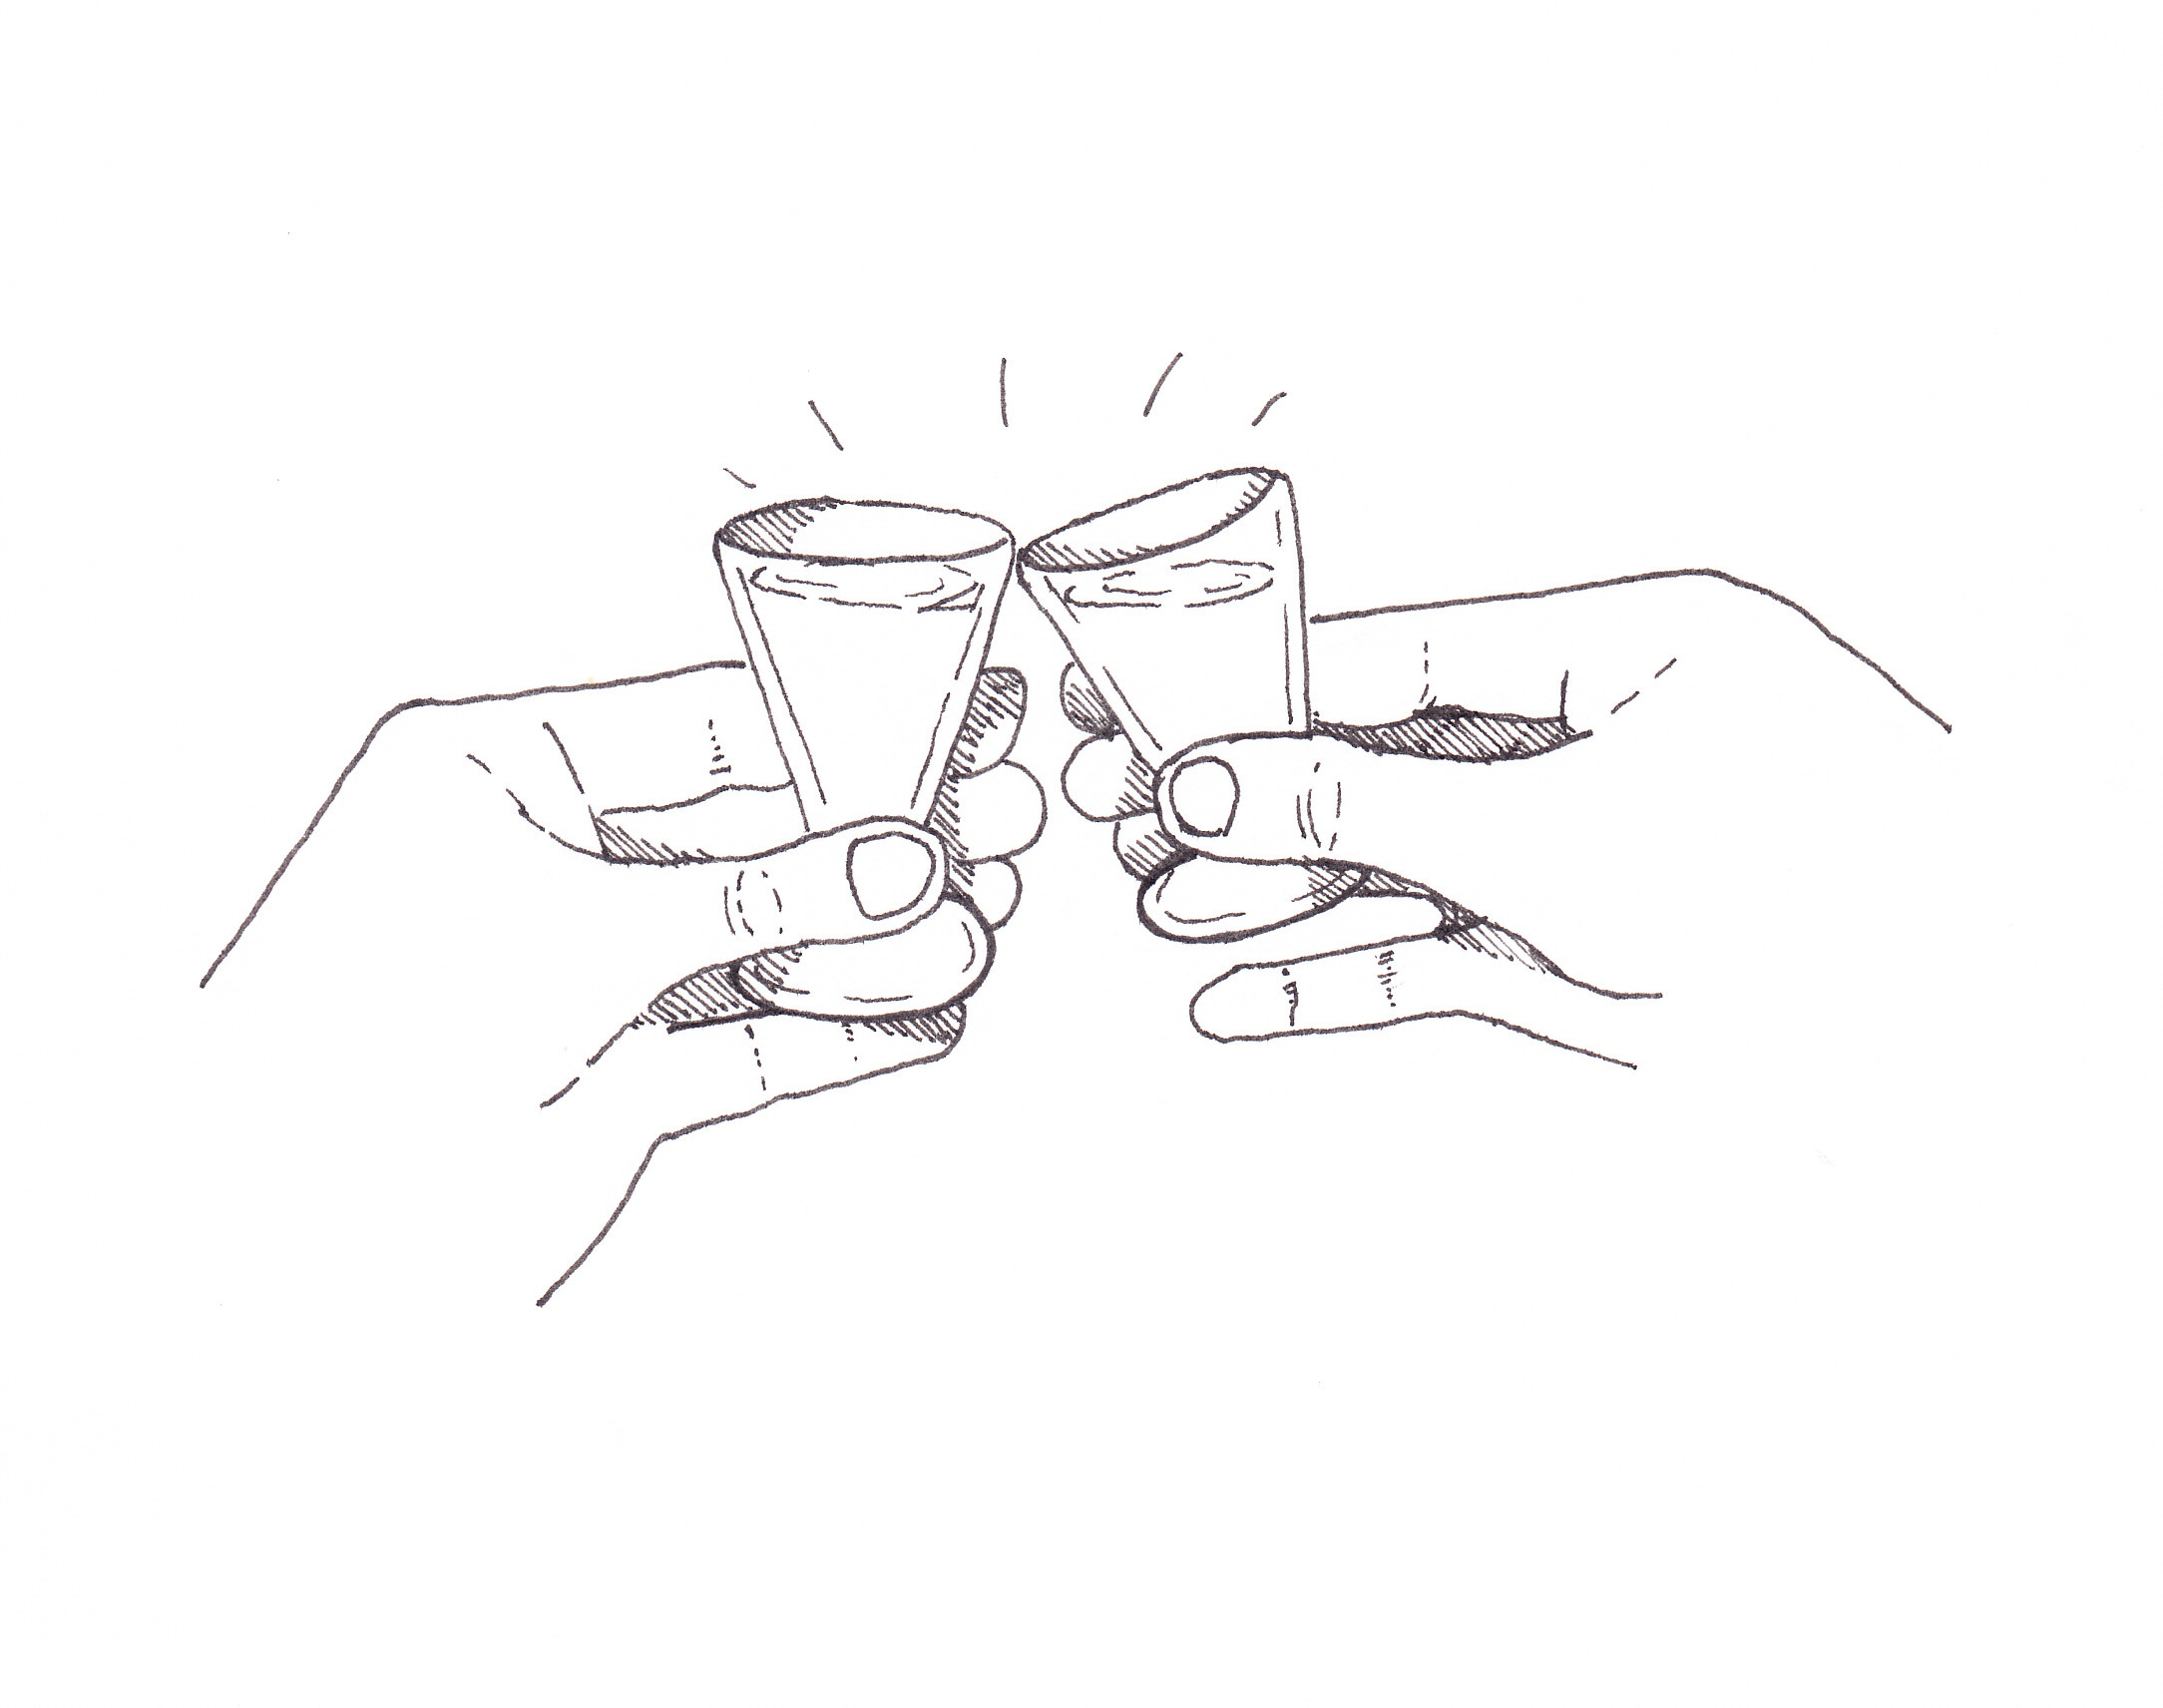
\includegraphics[width=5cm]{../bilder/skalandehander.jpg} 
\end{center}
\end{figure}
\clearpage
\beginsong{Rullaati, rullaati}[ 						
	index={Nu temperaturen är hög uti kroppen}]		
	
\beginverse*						
Nu temperaturen är hög uti kroppen, 
närmare 40 än 37.
 Men så skall det vara när ångan är oppe, 
och så är fallet uti detta nu. 
\endverse

\beginchorus				
Hej, rullaati rullaati rullaati rulla,
rullaati rullaati rullallalei! 
Hej, rullaati rullaati rullaati rulla,
rullaati rullaati rullallalei! 
\endchorus

\beginverse
Livet är kort som en barnunges tröja, 
ingenting kan vi väl göra åt det.
Men med vår sång kan bekymren vi röja, 
bort ifrån vardagens grådaskighet. 
\endverse	

\beginchorus
Hej rullaati...	
\endchorus

\beginverse
Snabbt flyktar ungdomens korta sekunder, 
skynda dig därför och räck mig din hand! 
Ej skall förgäves vi leva de stunder, 
då vi med sång knyter vänskapens band. 
\endverse	

\beginchorus
Hej rullaati...
\endchorus	
\endsong		

\clearpage
\beginsong{Sibbovisan}[ 							
	sr={Finska polkan},					
	index={Brännvini bränner}]		
	
\beginverse*						
Brännvini bränner, och bultar och dunkar, 
sibboborna huttar och klunkar,
tar sig en Hela, 
tar sig en Halva, 
Tersen och Kvarten och Kvinten på!
Tar det på allvar,
liksom ystra kalvar,
tar sig en Hela, 
tar sig en Halva,
Tersen och Kvarten och Kvinten på!
\endverse						

\beginverse				
En del har frågat, och somliga undrar:
Kan man ta starkt när det blixtrar och dundrar?
Kan man ta Helan, 
kan man ta Halvan,
Tersen och Kvarten och Kvinten på?
Svar till er alla:
Skåla när det knallar!
Pang, där gick Helan!
Pang, där gick Halvan!
Tersen och Kvarten och Kvinten på!
\endverse				
\endsong		

\clearpage
\beginsong{Sörnai gusha}[ 										
	index={Oon vain köyhä poika}]		
	
\beginverse*						
Sörnai gusha nietu Molotova
sörnai gusha herba Moskova.
:,: Njet, njet bonimal votvot risubuska,
dara zeva votvot harasoo. :,:
\endverse

\beginverse				
Isa Stalin ja äiti Grutzheva,
iski silmää gini hibragas.
:,: Oi-oi oisiba vodgaa ollut heillä,
oisi isgu gäynyd alemmas. :,:
\endverse

\beginverse
Siellä missä versoaapi vilja, 
siellä kasvoi kaunis Katjuska.
:,: Katjuskalla koimat on keuhkot,
baska haisee Nevan rannalla. :,:
\endverse

\beginverse
Oon vain köyhä kolhoosinainen,
ei oo mulla yhtään ystävää.
:,: Ei ole lehmää eikä ole lammasta,
eikä suussa yhtään hammasta. :,:
\endverse

\beginverse
Siperian lakeus on suuri,
Sonja siellä lunta lapioi.
:,: Sonjalla kävi hiton huono tuuri,
kun länsituuli uutta lunta toi. :,;
\endverse

\beginverse
Oon vain köyhä poika Petroskoista,
ei oo mulla yhtään ystävää. 
:,: Sirppi ja vasara ne taivahalla loistaa,
baska haisee, balalaikka soi. :,:
\endverse		
\endsong		

\clearpage
\beginsong{Strunt i sorger}[ 		
	by={T. Perret ?????????},					
	sr={},
	index={Hej dingelidong}]		
	
\beginverse*						
Strunt i sorger och bekymmer,
något roligt skall man ha.
När som livets afton skymmer,
då är det slut på det roliga.
Då går vi ut på vår balkong
och sjunger denna enkla sång:
Hej dingelidong,
HEJ dingelidong,
HEJ dingelidingelidong !
\endverse										
\endsong		

\beginsong{Tänään otetaan}[ 						
	sr={Joulu on taas},
	index={Idag ska vi ha}]		
	
\beginverse*						
:,: Tänään otetaan, tänään otetaan, 
helvetin paljon viinaa. :,:
:,: Huomenna on, huomenna on,
helvetin kova krapula. :,:
\endverse						

\beginverse				
:,: Idag ska vi ha, idag ska vi ha,
helvetes mycket brännvin. :,:
:,: Imorgon ska vi ha, imorgon ska vi ha,
helvetin kova krapula. :,:
\endverse
		

\beginverse				
:,: Täna võtame, täna võtame,
kuradima palju viina. :,:
:,: Homme meil on, homme meil on,
kuradima kova pohmakas. :,:

\endverse			
\endsong		

\clearpage

\beginsong{Tänk om jag hade lilla nubben}[ 					
	sr={Hej tomtegubbar}]	
	
\beginverse*						
Tänk om jag hade lilla nubben på ett snöre i halsen.
Tänk om jag hade lilla nubben på ett snöre i halsen.
Jag skulle dra den upp och ner,
så att den kändes som många fler.
Tänk om jag hade lilla nubben på ett snöre i halsen.
\endverse						

\vspace{5mm}	
\endsong		
		
\beginsong{Till spritbolaget}[ 		
	by={Georg Riedel},					
	sr={Du käre lille snickerbo}]		
	
\beginverse*						
Till spritbolaget ränner jag och bankar på dess port. 
Jag vill ha nå't som bränner bra och får mig skitfull fort.
Expediten sade godda', hur gammal kan min herre va'?
Har du nå't leg, ditt fula drägg? Kom hit tillbaks när du fått skägg!
\endverse						

\beginverse				
Men detta var ju inte bra, jag vill bli full ikväll.
Då kom jag på en bra idé, dom har ju sprit på Shell.
Många flaskor stod där på rad, hurra nu jag kan bli full och glad.
Den röda drycken rann sen ner, nu kan jag inte se nåt mer!
\endverse				
\endsong		

\clearpage
\beginsong{Tuborg}		
	
\beginverse*						
Tu tu tu Tuborg 
och ca ca ca Carlsberg 
det är den bästa 
pi pi pi pilsnern som jag vet 
\endverse						

\beginverse				
Tu tu tu Carlsberg 
och ca ca ca Tuborg 
det är det bästa 
pi pi pi ölet jag vet. 
\endverse

\beginverse
Tu ca pi Ölsner och 
pi ta ca bira 
det är den bästa 
ca pi tu lering som jag gjort.
\endverse
\endsong		

\begin{figure}[!b]
\begin{center}
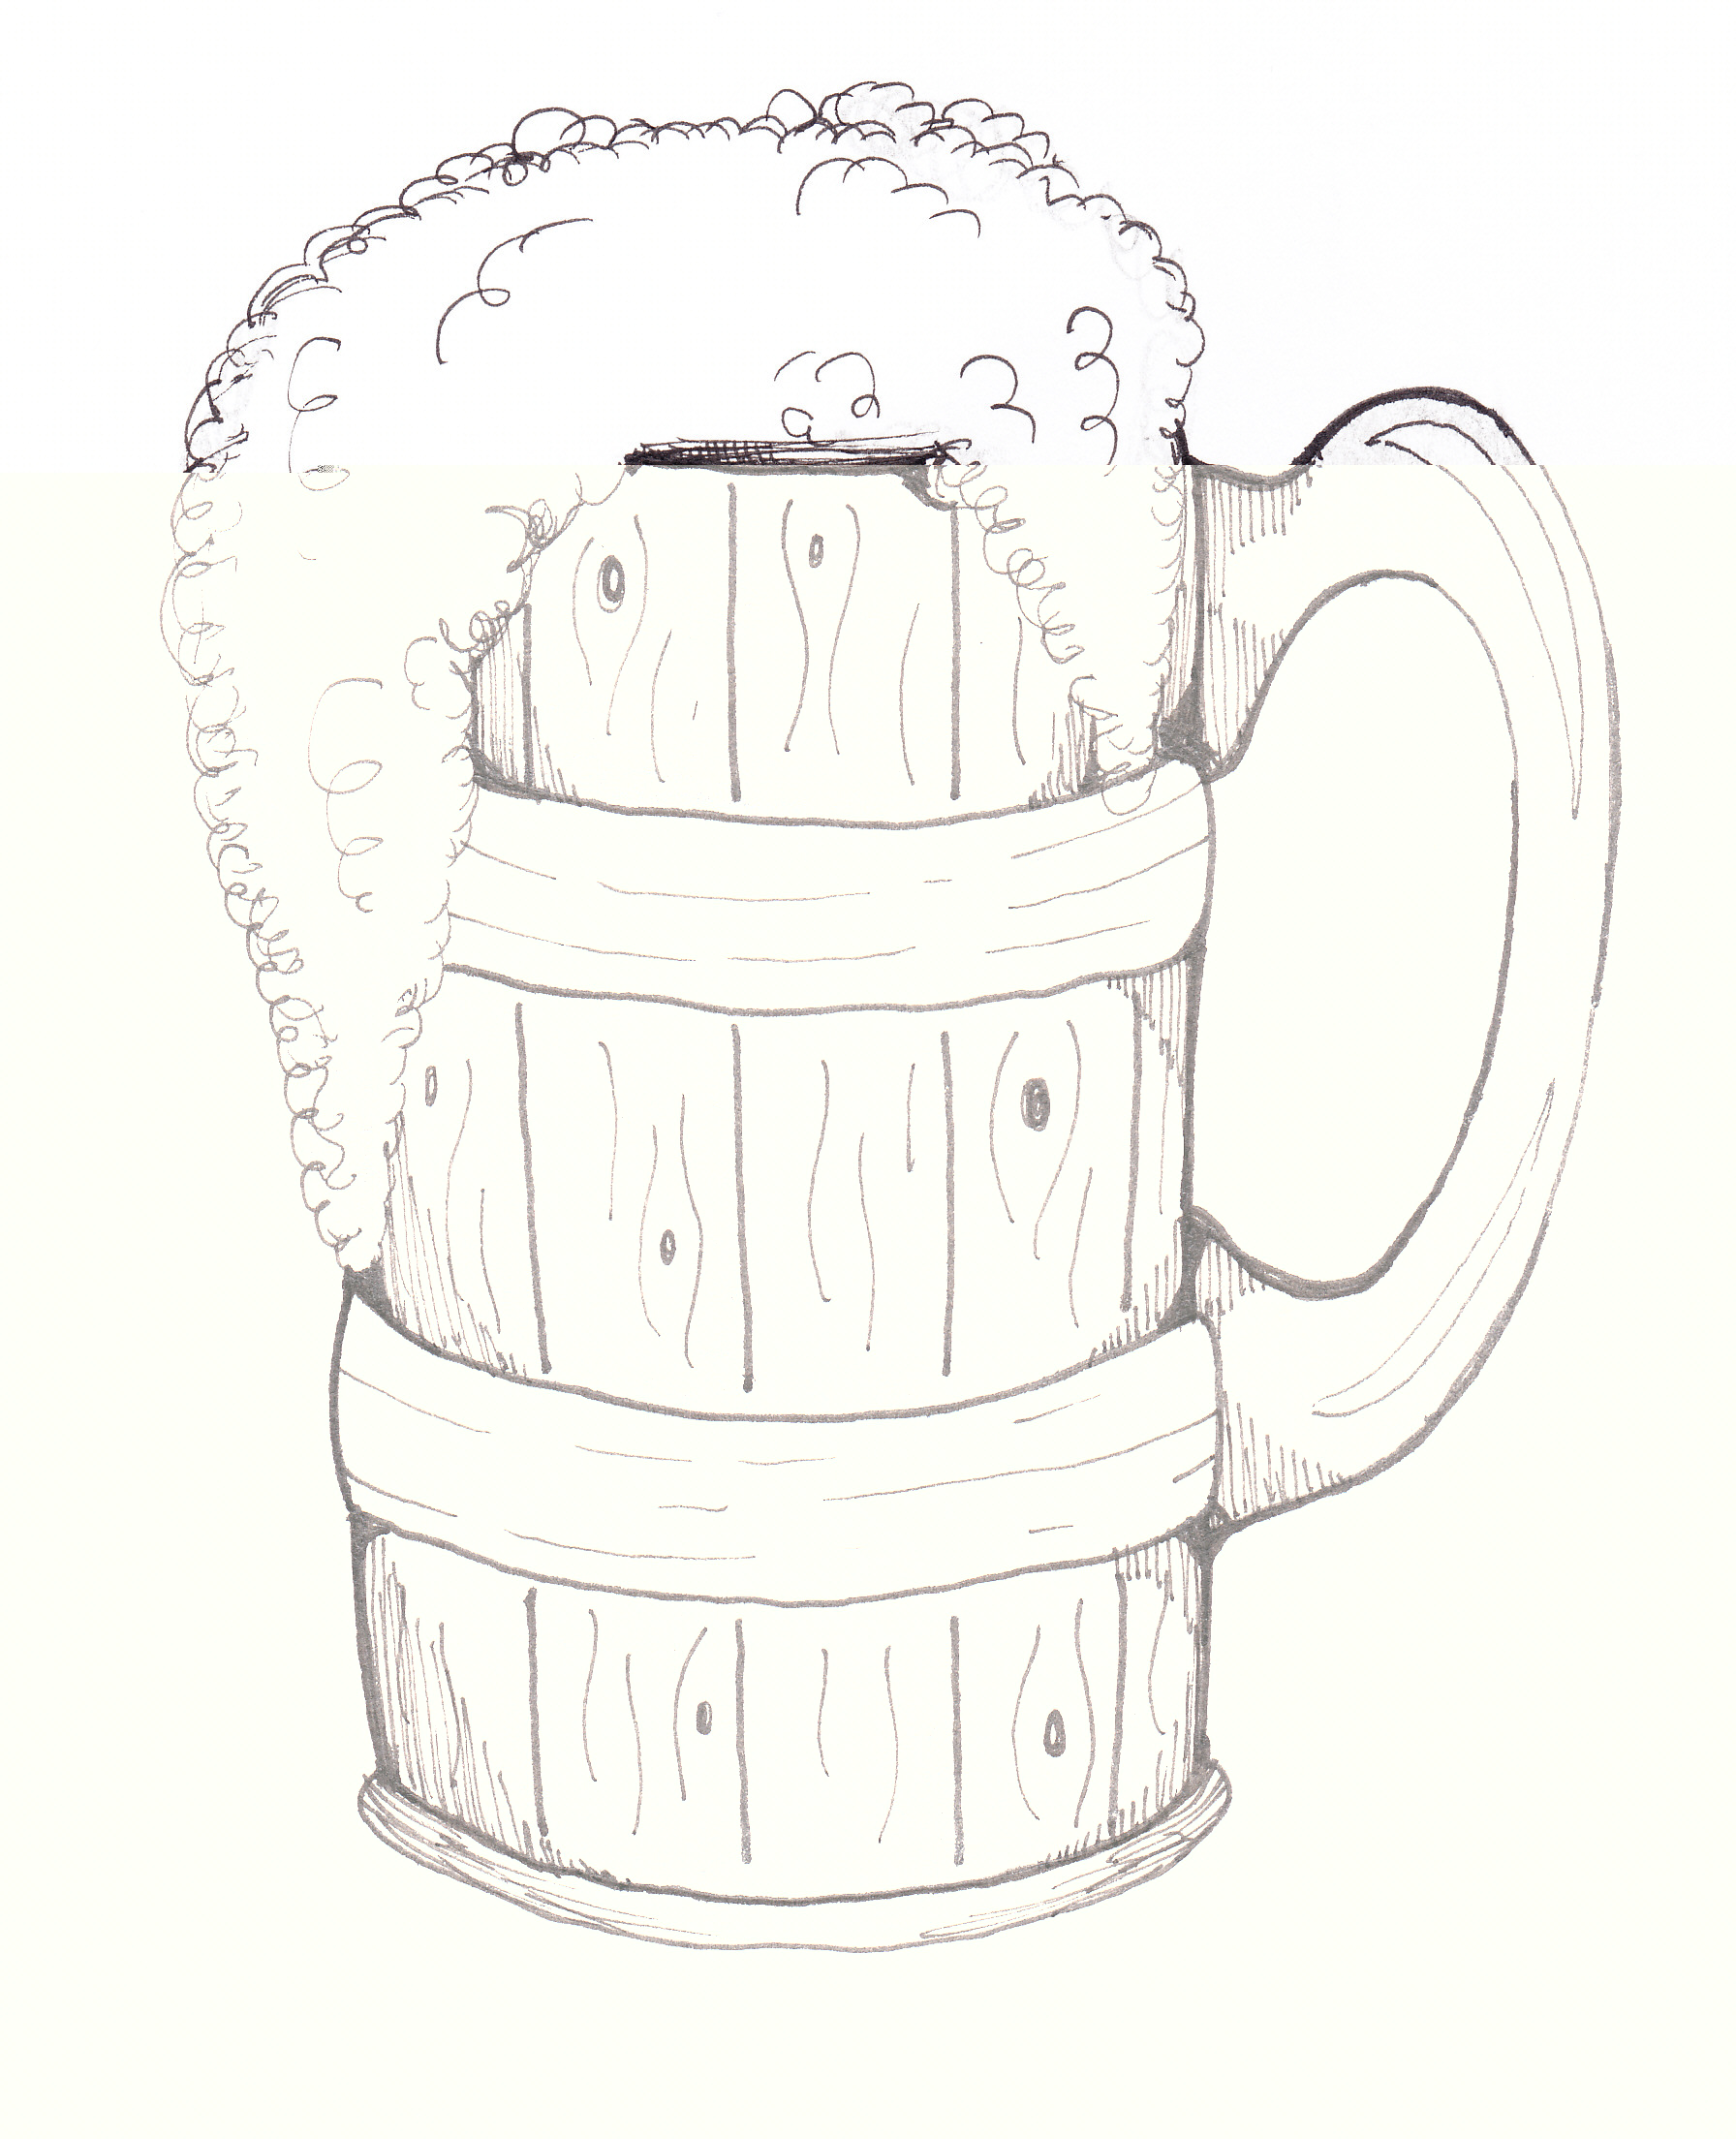
\includegraphics[width=30mm]{../bilder/stop.jpg} 
\end{center}
\end{figure}
\clearpage
\beginsong{Uti vår mage}[ 							
	sr={Uti vår hage},
	index={Kom Skåne och Aqua Vitae}]		
	
\beginverse*						
Uti vår mage där växa begär,
kom hjärtans kär.
Vill du mig något så träffas vi där. 
Kom Skåne och Aqua Vitae
kom O.P. och allt vad sprit ä'
kom ljuva Genever, kom Överste! 
\endverse										
\endsong		

\beginsong{Uti vårt barskåp}[ 						
	sr={Uti vår hage}]		
	
\beginverse*						
Uti vårt barskåp där råder en brist,
den är så trist,
men Alko måtte väl vekna till sist. 
Och då skall vi nog förgylla
vår vardag med liten fylla, 
för ingen vill sakna
god alkohol.
\endverse										
\endsong		

\clearpage

\beginsong{Där som sädesfälten}[ 						
	sr={Barndomshemmet},					
	index={Där som sädesfälten}] 
		
\beginverse*					
Där som sädesfälten böjer sig för vinden, 
står nån jävel där och böjer dem tillbaks!
\endverse									
\endsong				
\begin{figure}[!b]
\begin{center}
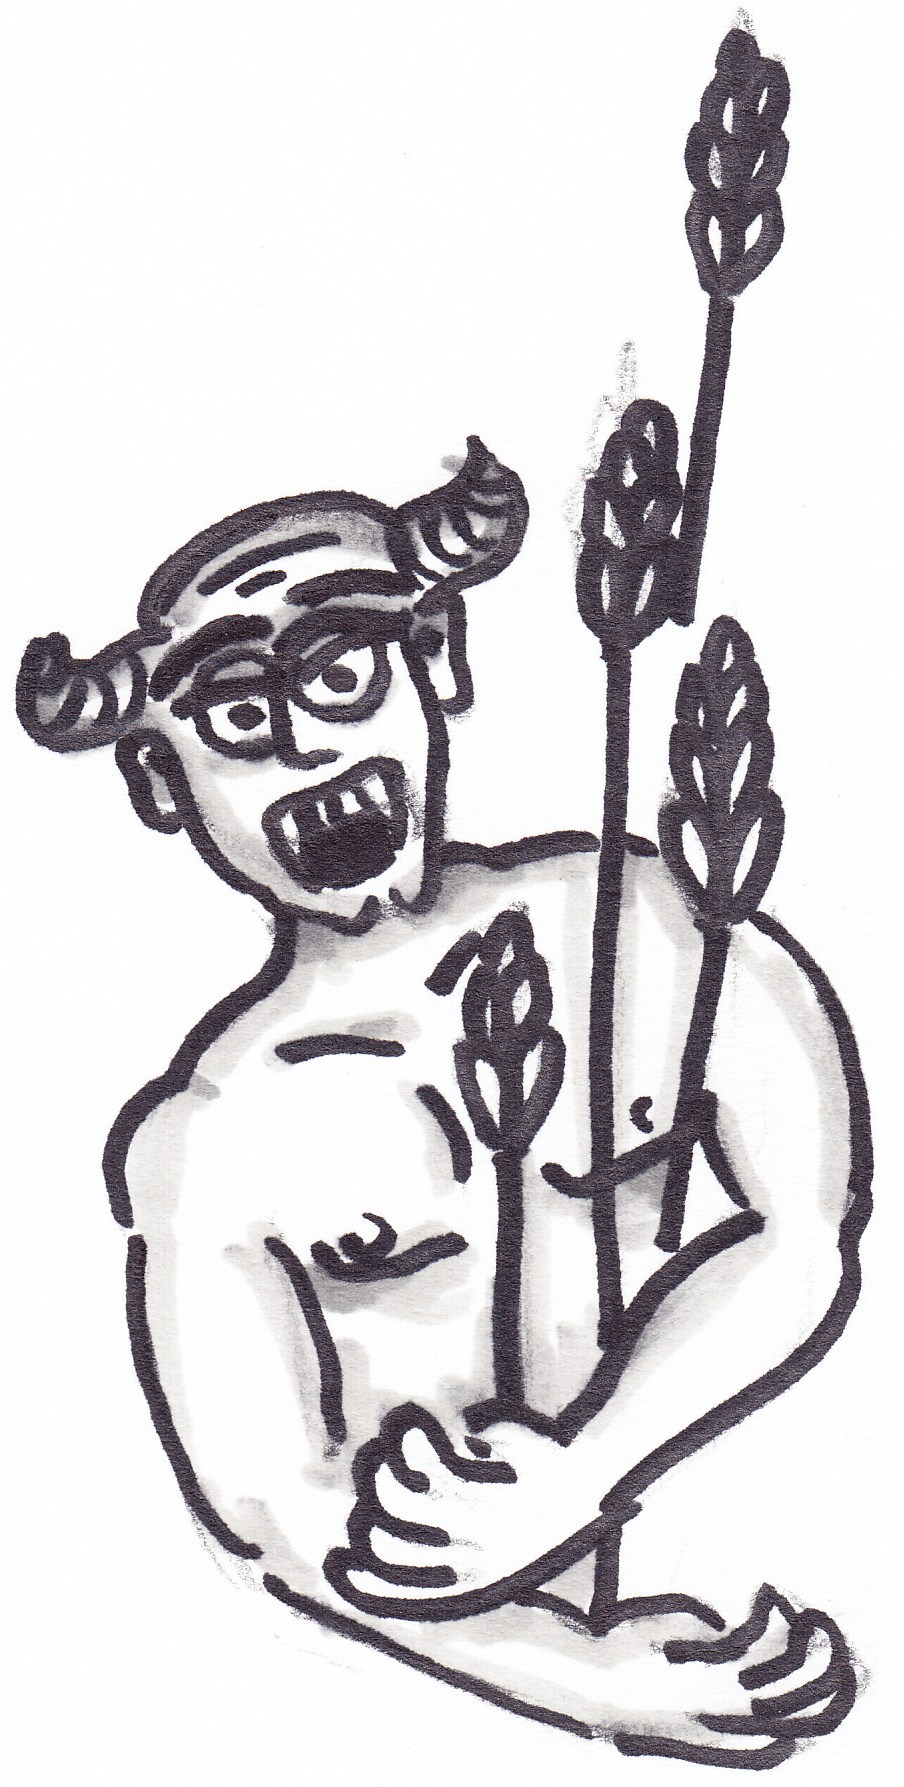
\includegraphics[width=3cm]{../bilder/javel.jpg} 
\end{center}
\end{figure}
\clearpage
\beginsong{Vem sade ordet}[ 							
	sr={Vårvindar friska}]		
	
\beginverse*						
Vem sade ordet ``skål'' här vid bordet,
viskande for det sällskapet kring.
Fattom kristallen, nubben är kall den,
stiger åt skallen, pling- planga- pling.
Käraste vänner, välkomna hit,
känn hur den doftar god akvavit.
Nu lilla hutten, går i kaputten,
skål lilla tutten, pling- planga- pling.
\endverse		

\vspace{5mm}								
\endsong		

\beginsong{Vodka, vodka}[ 							
	sr={Stenka Rasin},					
	index={Uppå väggen går en gädda}]		
	
\beginverse*						
Vodka, vodka vill jag dricka,
jag vill äta kaviar.
:,: Jag vill älska russki flicka,
jag vill spy i samovar! :,:
\endverse						

\beginverse				
Uppå väggen går en gädda, 
med långa ludna svarta ben.
:,: Men ni ska inte vara rädda,
ta en sup, och allt går väl! :,:
\endverse
				
\beginverse				
Vita möss, som går i taket,
råma hest och falla ner.
:,: Men ni ska inte vara rädda, 
ta en sup och allt går väl! :,:
\endverse	
\endsong	

\clearpage
% Exempel på färdig-formaterad sång till VN:s
% sångbok 2010.

% Denna fil kan användas som sådan, bara verserna,
% namnen och annan rådata behöver bytas ur fälten.
% Tecknet "%" markerar en kommentar som helt och 
% hållet ignoreras av programmet som läser filen.

% Spara den färdiga filen som 
% 'SangnamnUtanMellanslagEllerSkander.tex'
% t.ex. blir "Vid En Källa" till 
% 'VidEnKalla.tex'
% Varje sång blir en egen fil.

\beginsong{Öl, vin, sprit}[ 	% Börja sången här
	by={},	% Författare
	sr={Jenka}			% Melodi
	]		% Alternativa
			% sångnamn
	
\beginverse*		% Börja vers
Öl, vin, sprit och gammal finkel,
har fått mig att se i vinkel.
Därför hamnar inte supen i strupen 
utan i min hörapparat.
Va? Skåååål?
\endverse			% Sluta vers

\vspace{5mm}
\endsong			% Sluta sång

% Exempel på färdig-formaterad sång till VN:s
% sångbok 2010.

% Denna fil kan användas som sådan, bara verserna,
% namnen och annan rådata behöver bytas ur fälten.
% Tecknet "%" markerar en kommentar som helt och 
% hållet ignoreras av programmet som läser filen.

% Spara den färdiga filen som 
% 'SangnamnUtanMellanslagEllerSkander.tex'
% t.ex. blir "Vid En Källa" till 
% 'VidEnKalla.tex'
% Varje sång blir en egen fil.

\beginsong{Jag var full en gång}[ 	% Börja sången här
	by={},	% Författare
	sr={Flottarkärlek}]		% Alternativa
			% sångnamn
	
\beginverse*		% Börja vers
Jag var full en gång för länge sen,
på knäna kröp jag hem,
och på vägen träffa jag en elefant, elefant.
Elefanten börja pinka och jag trodde det var öl,
sedan dess har jag bli'tt kallad
jävla knöl, mera öl!
\endverse			% Sluta vers

\beginverse*		% Börja vers
Jag var full en gång för länge sen,
på knäna kröp jag hem,
varje dike var för mig ett vilohem, vilohem.
I varje hörn och varje vrå så hade jag en liten vän,
ifrån renat upp till 96 procent, mera sprit!
\endverse			% Sluta vers

\beginverse*		% Börja vers
Haderian haderej haderian hadera
Utan sprit går det inte bra
Haderian haderej haderian hadera
Lilla snapsen nu vi ta!
\endverse			% Sluta vers
\endsong			% Sluta sång

\clearpage
\beginsong{Vikingen}[
		sr={When Johnnie Comes Marching Home},
		index={En viking vill ha livets vann}]

\beginverse
En viking vill ha livets vann
Hurra, hurra!
Den hastigt i mitt svalg försvann
Hurra, hurra!
Till kalv, till oxe, till fisk, till fläsk
När kärringen bara dricker läsk
Då vill alla vikingar ha en besk. 
\endverse

\beginverse
När vi har druckit besken slut
Tragik, tragik!
Då bäres varje viking ut
som lik, som lik
och sen om vi vaknar vi sjunger en bit,
så korkar vi upp Skånes akvavit.
Skål för alla vikingar som kom hit!
\endverse
\endsong
\clearpage